\documentclass[class=article,10pt,crop=false]{standalone}
\usepackage{preamble}

\begin{document}
\begin{multicols}{2}[\section{Química}]
\subsection{Introducció}
Calor: $$dq=C_edT=nc_edT$$ {\footnotesize on $C_e$ és la capacitat calorífica; $n$, el nombre de mols, i $c_e$, la calor específica.}\newline
Llei dels gasos ideals: $$pV=nRT=Nk_BT$$ {\footnotesize on $R=k_BN_A=8,314\;J/(\text{mol }\cdot K)$ és la cons\-tant universal dels gasos ideals; $k_B=1,381\times 10^{-23}\;J/K$ és la constant de Boltzmann; $N_A=6,022\times10^{23}\;\text{mol}^{-1}$ és la constant d'Avogadro, i $N$ és el nombre de partícules. Els gasos reals compleixen aquesta equació al límit $p\to 0$.}\newline
Llei de Dalton: $$p_i:=x_ip$$ {\footnotesize on $p_i$ és la pressió parcial d'un gas; $x_i=\frac{n_i}{\sum_in_i}$ és la fracció molar, i $p$ és la pressió total.}\newline
Per a una mescla de gasos ideals es compleix: $$p_i=x_ip=\frac{n_iRT}{V}$$
Equació de Van der Waals (per a gasos reals): $$\left(p+\frac{an^2}{V^2}\right)\left(V-nb\right)=nRT$$ {\footnotesize on $a,b$ són paràmetres empírics.}\newline
Factor de compressibilitat $Z$: $$Z=\frac{pV}{nRT}$$ {\footnotesize Si $Z=1$, llavors es tracta d'un gas ideal. Si $Z>1$, dominen les forces repulsives sobre el gas. Si $Z<1$, dominen les forces atractives sobre el gas.}
\subsection{Formes de transferència d'energia}
Energia interna: 
$$dU=dW+dq\implies\Delta U=W+q$$ {\footnotesize on $W$ és el treball i $q$ és la calor intercanviats amb l'entorn.}\newline
\begin{figure}
    \centering
    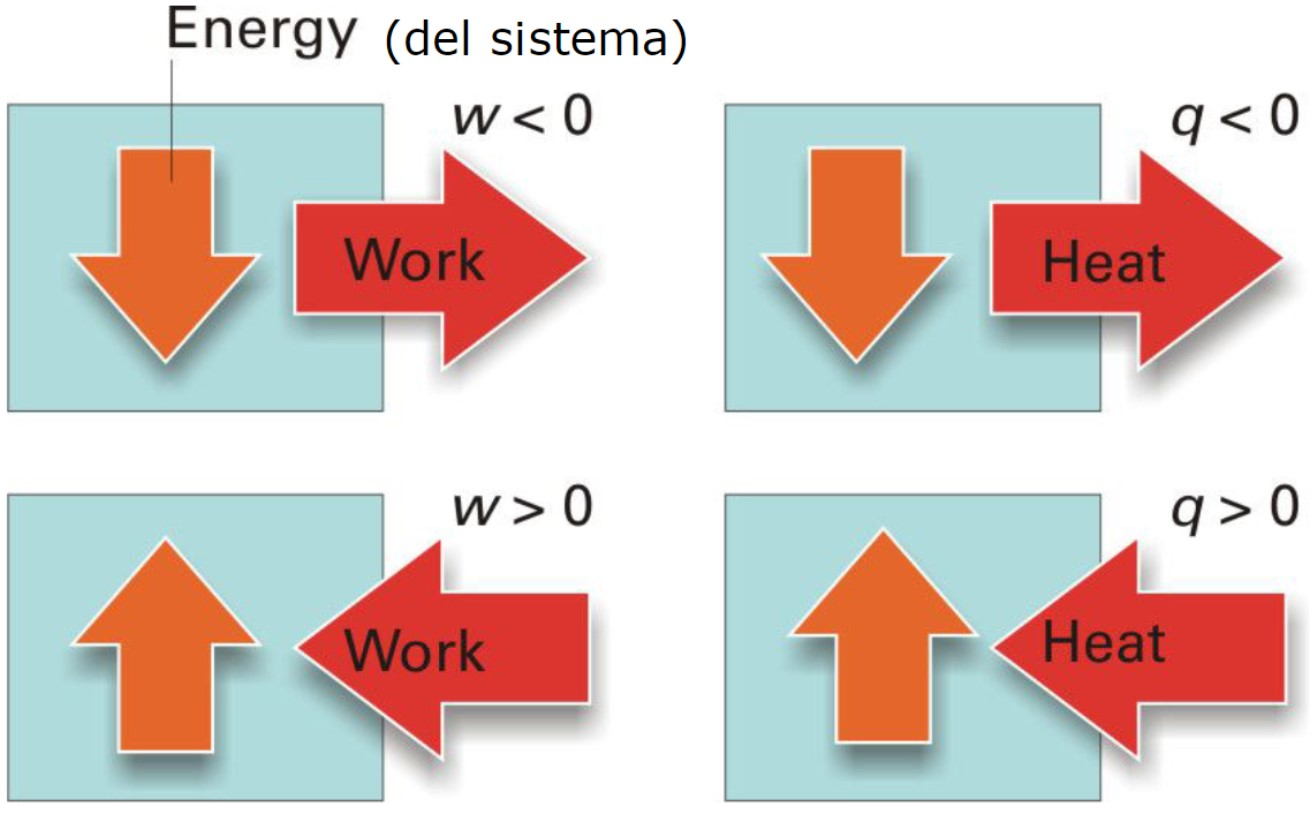
\includegraphics[width=4cm]{Physics/1st/Quimica/Imatges/workheat.jpg}
    \captionof{figure}{Criteri de signes del treball i calor interaccionant amb el sistema.}
    \label{fig:my_label}
\end{figure}
Entalpia: $$H=U+pV$$
Calor: $$q=nC(T_2-T_1)$$ {\footnotesize on $n$ és el nombre de mols i $C$ la calor específica.}
\begin{itemize}
    \item Volum constant: $$dU=dq_V\implies\Delta U=nC_V\Delta T$$
    \item Pressió constant: $$dH=dq_p\implies\Delta H=nC_p\Delta T$$
\end{itemize}
Relació de Mayer: $$C_p=C_V+R$$
Canvis d'estat en gasos ideals:
\begin{itemize}
    \item Cas general:
    \begin{align*}
        \Delta H&=nC_p(T_2-T_1)\\
        \Delta U&=nC_V(T_2-T_1)\\
        W&=-nR\int_{V_1}^{V_2}\frac{T}{V}dV
    \end{align*}
    \item Procés reversible isoterm (T=cte):
    \begin{align*}
        \Delta H&=0\\
        \Delta U&=0\\
        W&=-nRT\log\frac{V_2}{V_1}
    \end{align*}
    \item Procés reversible isobàric (p=cte):
    \begin{align*}
        \Delta H&=nC_p(T_2-T_1)\\
        \Delta U&=nC_V(T_2-T_1)\\
        W&=-p(V_2-V_1)
    \end{align*}
    \item Procés reversible isocor (V=cte):
    \begin{align*}
        \Delta H&=nC_p(T_2-T_1)\\
        \Delta U&=nC_V(T_2-T_1)\\
        W&=0
    \end{align*}
\end{itemize}
Definim l’entalpia de formació estàndard d’una substància pura a $T$ com $\Delta H^0$ per al procés de formació d’un mol de substància a partir dels seus elements separats en l’estat de referència, és a dir, en la seva forma més estable a temperatura $T$ i pressió $p=p^0=1$ bar.\newline
Entalpia estàndard d'una reacció: $$\Delta_rH^0=\sum_{\text{productes}}\nu\Delta_fH^0-\sum_{\text{reactius}}\nu\Delta_fH^0$$ {\footnotesize on $\nu$ és el coeficient estequiomètric de cada subs\-tàn\-cia.}\newline
Llei de Hess: $\Delta_rH^0$ d’una reacció és la suma de les entalpies estàndard de les reaccions en les quals es pot dividir.
Segons el signe de $\Delta_rH^0$, una reacció s'anomena exotèrmica ($\Delta_rH^0<0$) o endotèrmica ($\Delta_rH^0>0$).\newline
Entalpia d'enllaç:
$$\Delta_rH^0=\sum_{\substack{\text{enllaços}\\\text{trencats}}}\Delta_fH^0-\sum_{\substack{\text{enllaços}\\\text{formats}}}\Delta_fH^0$$
Llei de Kirchhoff: $$\Delta_rH_{T_2}^0=\Delta_rH_{T_1}^0+\int_{T_1}^{T_2}\Delta_rC_p^0dT$$ {\footnotesize on $\Delta_rC_p^0=\sum_{\text{productes}}\nu C_p^0-\sum_{\text{reactius}}\nu C_p^0$}
\subsection{Entropia}
Entropia:
\begin{gather*}
    dS=\frac{dq_\text{rev}}{T}\\
    \Delta S=\Delta S_{\text{sistema}}+\Delta S_{\text{entorn}}\geq 0
\end{gather*} {\footnotesize on $dq_\text{rev}$ és la calor transferida reversiblement.}\newline
Processos reversibles:
\begin{itemize}
    \item Procés adiabàtic ($dq_\text{rev}=0$):$$\Delta S=0$$
    \item Procés isotèrmic: $$\Delta S=\frac{\Delta H}{T}$$
    \item Escalfament a $p$ constant (isobàric): $$\Delta S=nC_p\log\frac{T_2}{T_1}$$
    \item Escalfament a $V$ constant (isocor): $$\Delta S=nC_V\log\frac{T_2}{T_1}$$
    \item Canvi d'estat d'un gas ideal: $$\Delta S=nC_V\log\frac{T_2}{T_1}+nR\log\frac{V_2}{V_1}$$
\end{itemize}
Distribució de Boltzmann: $$\frac{N_i}{N}=\frac{e^{-E_i/(k_BT)}}{\sum_ie^{-E_i/(k_BT)}}$$ {\footnotesize on $N_i$ és el nombre de partícules a l'estat $i$; $N$, el nombre total de partícules, i $E_i$, l'energia al nivell $i$.}\newline
Definició estadística d'entropia: $$\Delta S=k_B\log\frac{W_2}{W_1}=Nk_B\log\frac{V_2}{V_1}$$ {\footnotesize on $W_i$ és igual al nombre de microestats (maneres diferents de distribuir-se mantenint l’energia total constant) associats a un determinat macroestat del sistema i $N$ és el nombre de partícules.}\newline
Enunciat de Nerst-Simon (3r principi de la termodinàmica): Per a qualsevol substància pura tenim: $$\lim_{T\to0}S=0$$
Entropia absoluta: $$S(T)=\int_0^T\frac{C_p}{T}dT$$
Entropia estàndard de reacció: $$\Delta_rS_T^0=\sum_{\text{productes}}\nu S_{m,T,i}^0-\sum_{\text{reactius}}\nu S_{m,T,i}^0$$
Energia lliure de Gibbs: $$G=H-TS$$
Desigualtat de Clausius (per a un procés espontani a $p,T=$cte): $$\Delta G<0$$
Relacions:
\begin{gather*}
    dG=Vdp-SdT\\
    dU=TdS-pdV\\
    dH=TdS+Vdp
\end{gather*}
Energia lliure estàndard de reacció: \begin{gather*}
    \Delta_rG_T^0=\Delta_rH_T^0-T\Delta_rS_T^0\\
    \Delta_rG_T^0\leq 0\\
    \Delta_rG_T^0=\sum_{\text{prod.}}\nu\Delta_fG_{T,i}^0-\sum_{\text{reac.}}\nu\Delta_fG_{T,i}^0
\end{gather*}
\subsection{Canvis de fase}
La fase estable a temperatura $T$ és la que té $G$ molar menor.\newline
Regla de les fases: $$L+F=C+2$$
{\footnotesize on $L$ és el nombre de graus de llibertat independents que s’han de fixar per determinar l’estat d’un sistema; $F$, el nombre de fases, i $C$, el nombre de components.}\newline
\begin{figure}
    \centering
    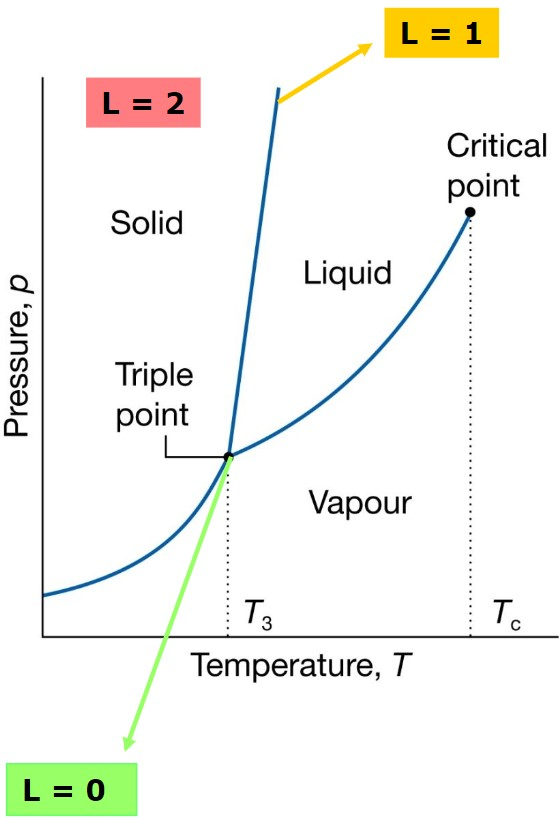
\includegraphics{Physics/1st/Quimica/Imatges/fases.jpg}
    \caption{Diagrama de fases d'una substància pura.}
\end{figure}
Equació de Clapeyron. Les línies de separació entre dues fases corresponen a valors de $p$ i $T$ on les dues fases coexisteixen, és a dir, estan en equilibri i, per tant, les seves $G_m$ són iguals: $$\frac{dp}{dT}=\frac{\Delta S_m}{\Delta V_m}=\frac{\Delta H_m}{T\Delta V_m}$$ {\footnotesize on $\Delta V_m=V_m^\alpha-V_m^\beta$,  $\Delta S_m=S_m^\alpha-S_m^\beta$ i $\alpha$ i $\beta$ són les diferents fases.}\newline
Equilibri sòlid-líquid. Temperatura de canvi de fase sòlid-líquid $T_2$ a una pressió $p_2$, coneixent $p_1$ i $T_1$:
$$p_2=p_1+\frac{\Delta H_{m,\text{fusió}}}{V_{m,\text{fusió}}}\log\frac{T_2}{T_1}$$
Equilibri líquid-gas. Suposant que el gas es comporta com un gas ideal $\rightarrow$ Equació de Clausius-Clapeyron: $$\frac{dp}{p}=\frac{\Delta H_{m,\text{vap}}}{RT^2}dT$$
Temperatura de canvi de fase líquid-gas $T_2$ a una pressió $p_2$, coneixent $p_1$ i $T_1$: $$\log\frac{p_2}{p_1}=-\frac{\Delta H_{m,\text{vap}}}{R}\left(\frac{1}{T_2}-\frac{1}{T_1}\right)$$
Equilibri sòlid-gas. Temperatura de canvi de fase sòlid-gas $T_2$ a una pressió $p_2$, coneixent $p_1$ i $T_1$: $$\log\frac{p_2}{p_1}=-\frac{\Delta H_{m,\text{sublim}}}{R}\left(\frac{1}{T_2}-\frac{1}{T_1}\right)$$
\subsection{Dissolucions}
Propietat molar: $$X_m=\frac{X(T,p,n_1,\ldots,n_i)}{n_\text{total}}$$
Propietat molar parcial: $$X_{m,i}=\left(\frac{\partial X}{\partial n_i}\right)_{T,p,n_{j\ne i}}$$
Formes d'expressar la concentració:
\begin{itemize}
    \item Fracció molar: $$x_i=\frac{n_i}{n}$$
    \item Molaritat: $$c_i=\frac{n_i}{V}$$ {\footnotesize on $V$ és el volum total de la dissolució.}
    \item Molalitat: $$m_i=\frac{n_i}{kg\text{ de dissolvent}}$$ 
    \item \% en pes: $$\frac{\text{g de solut}}{\text{100 g de dissolució}}$$
\end{itemize}
Potencial químic: $$\mu_i=\left(\frac{\partial G}{\partial n_i}\right)_{T,p,n_{j\ne i}}$$
Variació de $G_m=\mu^*$ a $T$ constant:
\begin{itemize}
    \item Gas ideal: $$\mu^*=\mu^0+RT\log\frac{p}{p_0}$$ {\footnotesize on $\mu^0$ és el potencial químic estàndard a $p=1$ bar.}
    \item Gas real: $$\mu^*=\mu^0+RT\log\frac{f}{p_0}$$ {\footnotesize on $f=\gamma p$ és la fugacitat i $\gamma$ és el coeficient de fugacitat.}
\end{itemize}
Mescla de gasos ideals: $$G_T=\sum_{i=1}^mn_i\left(\mu^0+RT\log\frac{p_i}{p_0}\right)$$
Propietat molar parcial: $$\mu_i(T,p)=\mu^0(T)+RT\log\frac{p_i}{p^0}$$
Mescla de gasos ideals: 
\begin{gather*}
    \Delta_\text{mix}H=0\\
    \Delta_\text{mix}G=nRT(x_A\log x_A+x_B\log x_B)\\
    \Delta_\text{mix}S=-nR(x_A\log x_A+x_B\log x_B)
\end{gather*} {\footnotesize on $x_A$ i $x_B$ són les fraccions molars de dos gasos ideals.}\newline
Una dissolució ideal és aquella en la quals les forces intermoleculars entre totes les espècies ($A, B,\ldots$) són iguals (interaccions $A-A=$ interaccions $B-B=$ interaccions $A-B$).\newline
Llei de Raoult: $$p_i=x_i^lp_i^*$$
Llei de Henry: $$p_B=x_B^lK_B$$ {\footnotesize on $K_B$ és la constant de Henry característica de cada solut.}\newline
Dissolució real: $$\mu_i=\mu_i^*+RT\log a_i$$ {\footnotesize on $a_i=\gamma_ix_i$ és l'activitat i $\gamma_i$ és el coeficient d'activitat.}
\subsection{Equilibri químic}
Condició d'equilibri material:
$$(dG)_{T,p}=\sum_\alpha\sum_{i=1}^k\mu_i^\alpha dn_i^\alpha=0$$ {\footnotesize on $\alpha$ és el nombre de fases.}\newline
Condició  d'equilibri químic (quan només tenim una fase): $$(dG)_{T,p}=\sum_{i=1}^k\mu_idn_i=0$$
Grau d'avanç $\xi$ d'una reacció: $$\Delta n=n_i-n_{i,0}=\xi\nu_i\implies dn_i=\nu_id\xi$$ {\footnotesize on $\nu_i$ són els coeficients estequiomètrics positius per als productes i negatius per als reactius.}\newline
Reacció:
\begin{itemize}
    \item En l'equilibri: $$\Delta_rG=\left(\frac{\partial G}{\partial \xi}\right)_{T,p}=\sum_{i=1}\mu_i\nu_i=0$$
    \item Fora de l'equilibri: $$\Delta_rG>0\text{  o  }\Delta_rG<0$$
\end{itemize}
Per a una reacció en l'equilibri: $$\Delta_rG^0+RT\log K_p=0$$ {\footnotesize on $K_p=\prod_i\left(\frac{p_i}{p_0}\right)^{\nu_i}$ és la constant d'equilibri.}
$$K_p=e^{-\Delta_rG^0/(RT)}$$
Constant en funció de fraccions molars: $$K_x=\prod_ix_i^{\nu_i}=K_p\left(\frac{p}{p^0}\right)^{-\Delta\nu}$$
Constant en funció de les concentracions: $$K_c=\prod_i\left(\frac{c_i}{c^0}\right)^{\nu_i}=K_p\left(\frac{c^0RT}{p^0}\right)^{-\Delta\nu}$$ {\footnotesize on $c_i\equiv\frac{n_i}{V}$ i $c^0\equiv1\;mol/L$ és la concentració estàndard.}\newline
Dependència amb la temperatura: $$\log\frac{K_p(T_2)}{K_p(T_1)}=\frac{-\Delta_rH^0}{R}\left(\frac{1}{T_2}-\frac{1}{T_1}\right)$$
Gasos no ideals:
$$K_p=\prod_i\left(\frac{f_i}{p_0}\right)^{\nu_i}=\prod_i(\gamma_i)^{\nu_i}\prod_i\left(\frac{p_i}{p_0}\right)^{\nu_i}$$ {\footnotesize on $f_i=\gamma_ip_i$ és la fugacitat i $\gamma_i$ és el coeficient de fugacitat.}\newline
Dissolucions no ideals:
$$K_c=\prod_i\left(\frac{a_i}{c_0}\right)^{\nu_i}=\prod_i(\gamma_i)^{\nu_i}\prod_i\left(\frac{c_i}{c_0}\right)^{\nu_i}$$ {\footnotesize on $f_i=\gamma_ip_i$ és l'activitat i $\gamma_i$ és el coeficient d'activitat.}\newline
Quocient de la reacció: $$\Delta_rG=RT\log\frac{Q_p}{K_p}$$ {\footnotesize on $Q_p=\prod_i\left(\frac{p_i}{p_0}\right)^{\nu_i}$ i quan la reacció està fora de l'equilibri. Si $Q_p>K_p\implies\Delta_rG>0\implies$ Reacció inversa (no espontània). I si $Q_p<K_p\implies\Delta_rG<0\implies$ Reacció directa (espontània).}
Equació de Van 't Hoff: $$\log\frac{K_p(T_2)}{K_p(T_1)}=\frac{-\Delta_rH^0}{R}\left(\frac{1}{T_2}-\frac{1}{T_1}\right)$$
\subsection{Equilibris iònics}
Reacció d'un àcid $A$ i una base $B$:
\begin{center}
    \ce{HA + H_2O <=> A^- + H_3O^+}\\
    \ce{B + H_2O <=> BH^+ + OH^-}
\end{center}
Constant d'acidesa i de basicitat: $$K_a=\frac{\ce{[A^-][H_3O^+]}}{\ce{[HA]}}\quad K_b=\frac{\ce{[BH^+][OH^-]}}{\ce{[B]}}$$
Relacions entre constants: $$K_aK_b=K_w=10^{-14}$$
pH i pOH:
\begin{gather*}
    \ce{pH}=-\log\ce{[H_3O^+]}\\
    \ce{pOH}=-\log\ce{[OH^-]}\\
    \ce{pH}+\ce{pOH}=14
\end{gather*}
pH en dissolucions tampó: $$\ce{pH}=\ce{p}K_a+\log\left(\frac{\ce{[A^-]}}{\ce{[HA]}}\right)$$ {\footnotesize on $\ce{p}K_a=-\log K_a$.}\newline
Constant de producte de solubilitat. Agafant com a exemple la reacció \ce{MgF_2 (s) <-> Mg^{2+} (aq) + 2F^- (aq)}: $$K_s=\ce{[Mg^{2+}][F^-]^2}$$ {\footnotesize on veiem que les concentracions dels ions que cons\-ti\-tu\-eix\-en el compost (\ce{MgF_2}) s'eleven als seus coeficients estequiomètrics.}\newline
La fem d'una pila: $$\xi=\xi_+-\xi_-=\xi_\text{càtode}-\xi_\text{ànode}$$
Reacció redox: $$\Delta G^0=-nF\xi^0$$ {\footnotesize on $n$ és el nombre d'electrons bescanviats; $F=N_Ae$ és la constant de Faraday, i $\xi^0$ és la fem estàndard de la pila que produeix la reacció redox.}\newline
Equació de Nernst: $$\xi=\xi^0-\frac{RT}{nF}\log Q$$
\subsection{Cinètica química}
La velocitat de la reacció es defineix com el canvi de la
composició del sistema en funció del temps. $$v_A=\frac{dn_A}{dt}$$ {\footnotesize on $n_A$ són els mols presents de la substància $A$.}
En general, la velocitat a la qual un reactiu es consumeix o un producte es forma és proporcional al coeficient estequiomètric.\newline
Si la reacció és elemental, el grau d'avanç de la reacció $\xi$ és: $$\xi=\frac{n_i-n_{i,t=0}}{\nu_i}$$ {\footnotesize on $n_i$ són els mols de la substància $i$; $n_{i,t=0}$, els mols de la substància $i$ en $t=0$, i $\nu_i$, el coeficient estequiomètric de la substància $i$.}\newline
Velocitat $v$ d'avanç de la reacció: $$v=\frac{d\xi}{dt}=-\frac{1}{a}v_A=\cdots=\frac{1}{\nu_i}\frac{dn_i}{dt}$$
Equació de velocitat: $$v=k_n[A]^\alpha[B]^\beta\cdots[L]^\lambda$$ {\footnotesize on els exponents $\alpha,\beta,\ldots,\lambda$ són enters o semienters. $\alpha$ és l'ordre de reacció respecte $A$; $\beta$ és l'ordre de reacció res\-pec\-te $B$;$\ldots$; $\lambda$ és l'ordre de reacció res\-pec\-te $L$, i $n=\alpha+\beta+\cdots+\lambda$ és l'ordre total de la reacció. La constant $k_n$ és la constant de ve\-lo\-ci\-tat d’ordre $n$ i és una mesura de la rapidesa de la reacció. Aquesta constant depèn de la temperatura.}\newline
Equacions integrades de velocitat en una reacció ($aA\rightarrow P$) elemental o complexa: $$v=-\frac{1}{a}\frac{d[A]}{dt}=k_n[A]^n$$
\begin{itemize}
    \item Ordre $n=1$: $$A=[A]_0e^{-akt}$$
    \item Ordre $n$ ($n\ne1$): $$\frac{1}{[A]^{n-1}}=\frac{1}{[A]^{n-1}_0}+a(n-1)kt$$
{\footnotesize on $[A]_0$ és la concentració inicial de la substància $A$.}
\end{itemize}
El període de semireacció és el temps necessari perquè la
concentració d’un determinat reactiu es redueixi a la meitat de la seva concentració inicial.\newline
Equació d'Arrhenius: $$k(T)=Ae^{-\frac{E_a}{RT}}$$ {\footnotesize on $A$ és el paràmetre preexponencial d'Arrhenius; $E_a$, l'energia d'activació de la reacció; R, la cons\-tant universal dels gasos ideals, i $T$, la tem\-pe\-ra\-tu\-ra.}
\subsection{Mecanismes de reacció}
\begin{itemize}
    \item Reaccions reversibles (\ce{A <=>[$k_1$][$k_{-1}$] B}, $\ce{[A]_0}=\ce{[A]_0}$, $\ce{[B]_0}=0$):
    \begin{gather*}
        \ce{[A]}=\frac{\ce{[A]_0}\left(k_{-1}+k_1e^{-(k_1+k_{-1})t}\right)}{k_1+k_{-1}}\\
        \ce{[B]}=\frac{k_1\ce{[A]_0}\left(1-e^{-(k_1+k_{-1})t}\right)}{k_1+k_{-1}}\\
        \frac{\ce{[B]_\infty}}{\ce{[A]_\infty}}=\frac{k_1}{k_{-1}}=K_\text{eq}
    \end{gather*}
    \item Reaccions consecutives (\ce{A ->[$k_1$] I ->[$k_2$] P}, $\ce{[A]_0}=\ce{[A]_0}$, $\ce{[I]_0}=\ce{[P]_0}=0$):
    \begin{gather*}
        \ce{[A]}=\ce{[A]_0}e^{-k_1t}\\
        \ce{[I]}=\frac{k_1\ce{[A]_0}\left(e^{-k_1t}-e^{-k_2t}\right)}{k_2-k_1}\\
        \begin{split}
        \ce{[P]}=\ce{[A]_0}\left[1+\frac{1}{k_2-k_1}\left(k_1e^{-k_1t}-\right.\right.\\\left.\left.-k_2e^{-k_2t}\right)\right]
        \end{split}
    \end{gather*}
    \item Reaccions paral·leles o competitives (\ce{A ->[$k_1$] P_1} \ce{A ->[$k_2$] P_2} \ce{A ->[$k_3$] P_3}, $\ce{[A]_0}=\ce{[A]_0}$, $\ce{[P_i]_0}=0$):
    \begin{gather*}
        \ce{[A]}=\ce{[A]_0}e^{-k_Tt}\\
        \ce{[P_i]}=\frac{k_i}{k_T}\ce{[A]_0}\left(1-e^{-k_Tt}\right)
    \end{gather*}
    {\footnotesize on $k_T=k_1+k_2+k_3$.}\newline
    Mètodes aproximats:
    \begin{itemize}
        \item Aproximació de l'estat es\-ta\-ci\-o\-na\-ri:
        \begin{itemize}
            \item \ce{A ->[$k_1$] I ->[$k_2$] P} ($\ce{[A]_0}=\ce{[A]_0}$, $\ce{[I]_0}=\ce{[P]_0}=0$ i $k_2>>k_1$):
            \begin{gather*}
                \ce{[A]}=\ce{[A]_0}e^{-k_1t}\\
                \ce{[I]_{EE}}=\frac{k_1}{k_2}\ce{[A]_0}e^{-k_1t}\\
                \ce{[P]_{EE}}=\ce{[A]_0}\left(1-e^{-k_1t}\right)
            \end{gather*}
            \item \ce{A <->[$k_1$][$k_{-1}$] I ->[$k_2$] P} ($\ce{[A]_0}=\ce{[A]_0}$, $\ce{[I]_0}=\ce{[P]_0}=0$ i $k_2\text{ o }k_{-1}>>k_1$):
            \begin{gather*}
                \ce{[I]_{EE}}=\frac{k_1}{k_{-1}+k_2}\ce{[A]_0}\\
                v=\frac{d\ce{[P]}}{dt}=k_2\ce{[I]}=\frac{k_2k_1\ce{[A]_0}}{k_{-1}+k_2}
            \end{gather*}
        \end{itemize}
        \item Aproximació de l'equilibri:
        \begin{itemize}
            \item \ce{A <->[$k_1$][$k_{-1}$] I ->[$k_2$] P} ($\ce{[A]_0}=\ce{[A]_0}$, $\ce{[I]_0}=\ce{[P]_0}=0$ i $k_1$ i $k_{-1}>>k_2$):
            \begin{gather*}
                \ce{[I]_e}=\frac{k_1}{k_{-1}}\ce{[A]_0}\\
                v=\frac{d\ce{[P]}}{dt}=k_2\ce{[I]}=\frac{k_2k_1\ce{[A]_0}}{k_{-1}}
            \end{gather*}
        \end{itemize}
    \end{itemize}
\end{itemize}
\end{multicols}
\end{document}